\documentclass[a4paper]{article}


\usepackage[T1]{fontenc}
\usepackage[utf8]{inputenc}
\usepackage{mathptmx}

%\usepackage{ngerman}	% Sprachanpassung Deutsch

\usepackage{graphicx}
\usepackage{geometry}
\geometry{a4paper, top=15mm}

\usepackage{subcaption}
\usepackage[shortlabels]{enumitem}
\usepackage{amssymb}
\usepackage{amsthm}
\usepackage{mathtools}
\usepackage{braket}
\usepackage{bbm}
\usepackage{graphicx}
\usepackage{float}
\usepackage{yhmath}
\usepackage{tikz}
\usepackage{algorithm}
\usepackage{algpseudocode}
\usetikzlibrary{patterns,decorations.pathmorphing,positioning}
\usetikzlibrary{calc,decorations.markings}

\newcommand{\eps}{\varepsilon}

\usepackage[backend=biber, sorting=none]{biblatex}
\addbibresource{uni.bib}

\usepackage[framemethod=TikZ]{mdframed}

\tikzstyle{titlered} =
    [draw=black, thick, fill=white,%
        text=black, rectangle,
        right, minimum height=.7cm]


\usepackage[colorlinks=true,naturalnames=true,plainpages=false,pdfpagelabels=true]{hyperref}
\usepackage[parfill]{parskip}
\usepackage{lipsum}


\usepackage{tcolorbox}
\tcbuselibrary{skins,breakable}

\pagestyle{myheadings}

\markright{Popović\hfill Tensor Methods \hfill}


\title{University of Vienna\\ Faculty of Mathematics\\
\vspace{1cm}TENSOR METHODS FOR DATA SCIENCE AND SCIENTIFIC COMPUTING
}
\author{Milutin Popovic}

\begin{document}
\maketitle
\tableofcontents
\section{Assignment 5}
\subsection{Truncated TT-MPS}
Given an MPS-TT factorization $U_1, \dots ,U_d$ of $A \in
\mathbb{R}^{n_1\times \cdots \times n_d}$, with ranks $p_1, \dots, p_{d-1}\
\in \mathbb{N}$, we will produce a MPS-TT approximation of ranks not
exceeding $r_1, \dots, r_{d-1}$ with factors $V_1, \dots, V_d$ of
quasioptimal accuracy in the Forbenius norm.


\begin{algorithm}[H]
  \caption{rank truncation MPS-TT}\label{alg: hosvd}
\begin{algorithmic}
    \State $\tilde{U_1} \gets U_1$
    \For{$k = 1, \dots, d-1$}
        \State $\tilde{U}_k \gets \text{reshape}\left(\tilde{U}_k, (p_{k-1} \cdot n_k, r_k\right)$

        \State $\bar{U}_k \gets \hat{P}_k \hat{\Sigma}_k \hat{W}^*_k$
        \Comment{rank- $r_k$ T-SVD of $\tilde{U}_k$}

        \State $\hat{Q}_k \gets \text{reshape}\left(\hat{P}_k, (p_{k-1}, n_k,
        r_k) \right)$

        \State $\hat{Z}_k \gets \text{reshape}\left(\hat{\Sigma}_k \hat{W}^*_k,
            (r_{k}, 1, p_k) \right)$

        \State $(\tilde{U}_{k+1})_{\beta_k,i_{k+1},\alpha_{k+1}} \gets
        \sum_{\alpha_k = 1}^{r_k} (\hat{Z}_k)_{\beta_k, 1, \alpha_k}
            (U_{k+1})_{\alpha_k, i_{k+1}, \alpha_{k+1}}$
        \State $\text{save}(\hat{Q_k})$
    \EndFor
    \State $\text{save}\left(\tilde{U}_d\right)$
\end{algorithmic}
\end{algorithm}
\subsection{TT-MPS arithmetic}
\subsubsection{Addition}
Consider two tensors $U$ and $V$ of size $n_1 \times \cdots \times n_d \ \in
\mathbb{N}$ for $d \in \mathbb{N}$, with TT-MPS factorization $U_k$ with rank
$p_k$ and $V_k$ with rank $q_k$ respectively (for $k \in \{1, \dots ,d-1\}$).
Then TT-MPS factorization of $W = U + V$ can be calculated without
evaluating $U$ or $V$, just by using $U_1, \dots, U_{d}$ and $V_1, \dots,
V_d$ by the following
\begin{align}
    W &= U_1 \bowtie \cdots \bowtie U_d + V_1 \bowtie \cdots \bowtie V_d
    =\nonumber\\
      &= \begin{bmatrix}U_1 & V_1\end{bmatrix} \bowtie
      \begin{bmatrix} U_2 \bowtie \cdots \bowtie U_d  \\  V_2 \bowtie \cdots
      \bowtie V_d  \end{bmatrix} =\nonumber\\
      &= \cdots =\nonumber\\
      &=\begin{bmatrix}U_1 & V_1\end{bmatrix} \bowtie \begin{bmatrix} U_2 &
    0\\ 0& V_2 \end{bmatrix} \bowtie \cdots \bowtie \begin{bmatrix} U_{d-1} &
    0\\ 0& V_{d-1} \end{bmatrix} \bowtie \begin{bmatrix} U_d \\ V_d
\end{bmatrix} =\nonumber\\
        &= W_1 \bowtie \cdots \bowtie W_d,
\end{align}
where $W$ has a decomposition of ranks $(p_1 + q_1), \dots, (p_{d-1}
q_{d-1})$. The construction of these matrices and vectors can be done by
initializing the $W_k$ and then slicing for $U_k$ and $V_k$ in the second
dimension, meaning $n_k$. Thereby for the $k$-th ($2\leq k \leq d-2$) step we would have
\begin{align}
    (W_k)_{:, i_k, :} = \begin{bmatrix} (U_k)_{:, i_k, :} & 0 \\
                                        0 & (V_k)_{:, i_k, :}
                        \end{bmatrix} \;\;\;\; \forall i_k \in \{1, \dots,
                        n_k\}.
\end{align}
For the first step we have $p_0 = q_0 = 1$ and thereby
\begin{align}
    (W_1)_{:, i_1, :} = \begin{bmatrix} (U_1)_{1, i_1,:} & (V_1)_{1, i_1, :}
    \end{bmatrix} \;\;\;\;\; \forall i_1 \in \{1, \dots, n_1 \}.
\end{align}
And for the $k=d$-th step we have $p_d = q_d = 1$ and thereby
\begin{align}
    (W_d)_{:, i_d, :} = \begin{bmatrix} (U_d)_{:, i_d,1} \\ (V_d)_{:, i_d, 1}
    \end{bmatrix} \;\;\;\;\; \forall i_d \in \{1, \dots, n_d \}.
\end{align}
This concludes the construction of the algorithm for addition
\subsubsection{Hadamard Product}
Now consider again two tensors $U$ and $V$ of size $n_1 \times \cdots \times n_d \ \in
\mathbb{N}$ for $d \in \mathbb{N}$, with TT-MPS factorization $U_k$ with rank
$p_k$ and $V_k$ with rank $q_k$ respectively (for $k \in \{1, \dots ,d-1\}$).
Then TT-MPS factorization of $W = U \otimes V$ can be calculated without
evaluating $U$ or $V$, just by using $U_1, \dots, U_{d}$ and $V_1, \dots,
V_d$ by the following
\begin{align}
    W_{i_1, \dots, i_d} &= \sum_{\alpha_1 = 1}^{q_1} \cdots \sum_{\alpha_{d-1}
    = 1}^{q_{d-1}} \prod_{k=1}^d U_k(\alpha_{k-1}, i_k, \alpha_k) \cdot
    \sum_{\beta_1 = 1}^{q_1} \cdots \sum_{\beta_{d-1}
        = 1}^{q_{d-1}} \prod_{k=1}^d V_k(\beta_{k-1}, i_k, \beta_k)
        =\nonumber\\
        =&
    \sum_{\gamma_1 = 1}^{r_1} \cdots \sum_{\gamma_{d-1}
        = 1}^{r_{d-1}} \prod_{k=1}^d W_k(\gamma_{k-1}, i_k, \gamma_k).
\end{align}
Thereby the factors $W_k$ can be calculated with the factor wise product
\begin{align}
    W_k(\alpha_{k-1}\beta{k-1}, i_k, \alpha_k\beta_k) = U_k(\alpha_{k-1},
    i_k, \alpha_k) \cdot V_k(\beta_{k-1}, i_k, \beta_k),
\end{align}
for all $\alpha_{k} \in \{1, \dots, p_{k}\}$ and $\beta_k \in \{1, \dots,
q_k\}$ and $p_0 = p_d = q_0 = q_d = 1$. Where the TT-MPS calculated by the
algorithm is of ranks $(p_1q_1), \dots, (p_{d-1} q_{d-1})$.

The computer reads in slices and Kronecker products
\begin{align}
    (W_k)_{:, i_k, :} = (U_k)_{:, i_k, :} \otimes (V_k)_{:, i_k, :}
    \;\;\;\;\;\; \forall i_k \in \{1, \dots, n_k\}.
\end{align}
\subsubsection{Matrix Vector product}
Now consider $A\in \mathbb{R}^{n_1\cdots n_d \times m_1 \cdots m_d}$ and
$u \in \mathbb{R}^{m_1 \cdots m_d}$. The TT-MPS factorization of $A$ is $A_k
\in \mathbb{R}^{p_{k-1} \times n_k \times m_k \times q_k}$ and the TT-MPS
factorization of $U$ is $U_k \in \mathbb{R}^{q_{k-1} \times m_k \times q_k}$.
The TT-MPS factors $W_k$ of $w = A\cdots u$ can be explicitly calculated with
\begin{align}
    W_{i_1,\dots, i_d} &= \sum_{j_1,\dots,j_d} A_{i_1\cdots i_d, j_1\cdots
        j_d} U_{j_1\cdots j_d}\nonumber \\
        &= \sum_{j_1, \dots, j_d}
        \sum_{\alpha_1=1}^{p_1} \cdots \sum_{\alpha_{d-1}=1}^{p_{d-1}}
        \prod_{k=1}^d A_k(\alpha_{k-1}, i_k, j_k, \alpha_k) \cdot
        \sum_{\beta_1=1}^{q_1} \cdots \sum_{\beta_{d-1}=1}^{q_{d-1}}
        \prod_{k=1}^d U_k(\beta_{k-1} j_k, \beta_k) \cdot \nonumber\\
        &= \sum_{\alpha_1\beta_1} \cdots \sum_{\alpha_{d-1}\beta_{d-1}}
        \prod_{k=1}^{d} \left(
        \sum_{j_k}^{n_k} A_k(\alpha_{k-1}, i_k, j_k, \alpha_k)
        U_K(\beta_{k-1}, j_k, \beta_k)
        \right) \nonumber \\
        &= \sum_{\gamma_1}^{r_1} \cdots \sum_{\gamma_{d-1}}^{r_{d-1}}
        \prod_{k=1}^{d} W_k(\gamma_{k-1}, i_k, \gamma_k),
\end{align}
for $r_k = q_k \cdot p_k$.
The computer reads
\begin{align}
    (W_k)_{:, i_k, :} = \sum_{j_k=1}^{n_k} (A_k)_{:, i_k, j_k, :} \otimes
    (U_k)_{:, j_k, :} \;\;\;\;\; \forall i_k \in \{1, \dots, n_k\}
\end{align}
for all $k = 1,\dots, d$
\subsection{Testing}
Consider the grid for $n=51$
\begin{align}
    t_i = 2\frac{i-1}{n-1} - 1 \;\;\;\;\; i = 1, \dots ,n
\end{align}
for the tensors $X, Y \in \mathbb{R}^{n\times n\times n\times n}$ given by
\begin{align}
    x_{i_1,\dots, i_4} &= T_p\left(\sum_{k=1}^4 \frac{t_{i_k}}{4}\right) \\
    y_{i_1,\dots, i_4} &= T_q\left(\sum_{k=1}^4 \frac{t_{i_k}}{4}\right) \\
\end{align}
for $p, q \in \mathbb{N}_0$ and $T_r$ is the Chebyshev polynomial for a $k
\in \mathbb{N}_0$. The Chebyshev polynomials are defined by
\begin{align}
    T_r(x) = \begin{cases}
        \cos(r\cdot\text{arccos}(x)) & \;\;\;\;\; |x| \leq 1\\
        \cosh(r\cdot\text{arccosh}(x))&\;\;\;\;\; x \geq 1\\
        (-1)^r\cosh(r\cdot\text{arccosh}(x))&\;\;\;\;\; x \leq -1
            \end{cases}.
\end{align}
Additionally we define
\begin{align}
    S := X + Y\\
    Z := X \otimes Y.
\end{align}
The following figures show for $(p, q) = 3,4$ and $(p, q) = 5,7$ the TT-MPS
unfolding singular values of tensors $X, Y, S, Z$.
\begin{figure}[H]
    \centering
    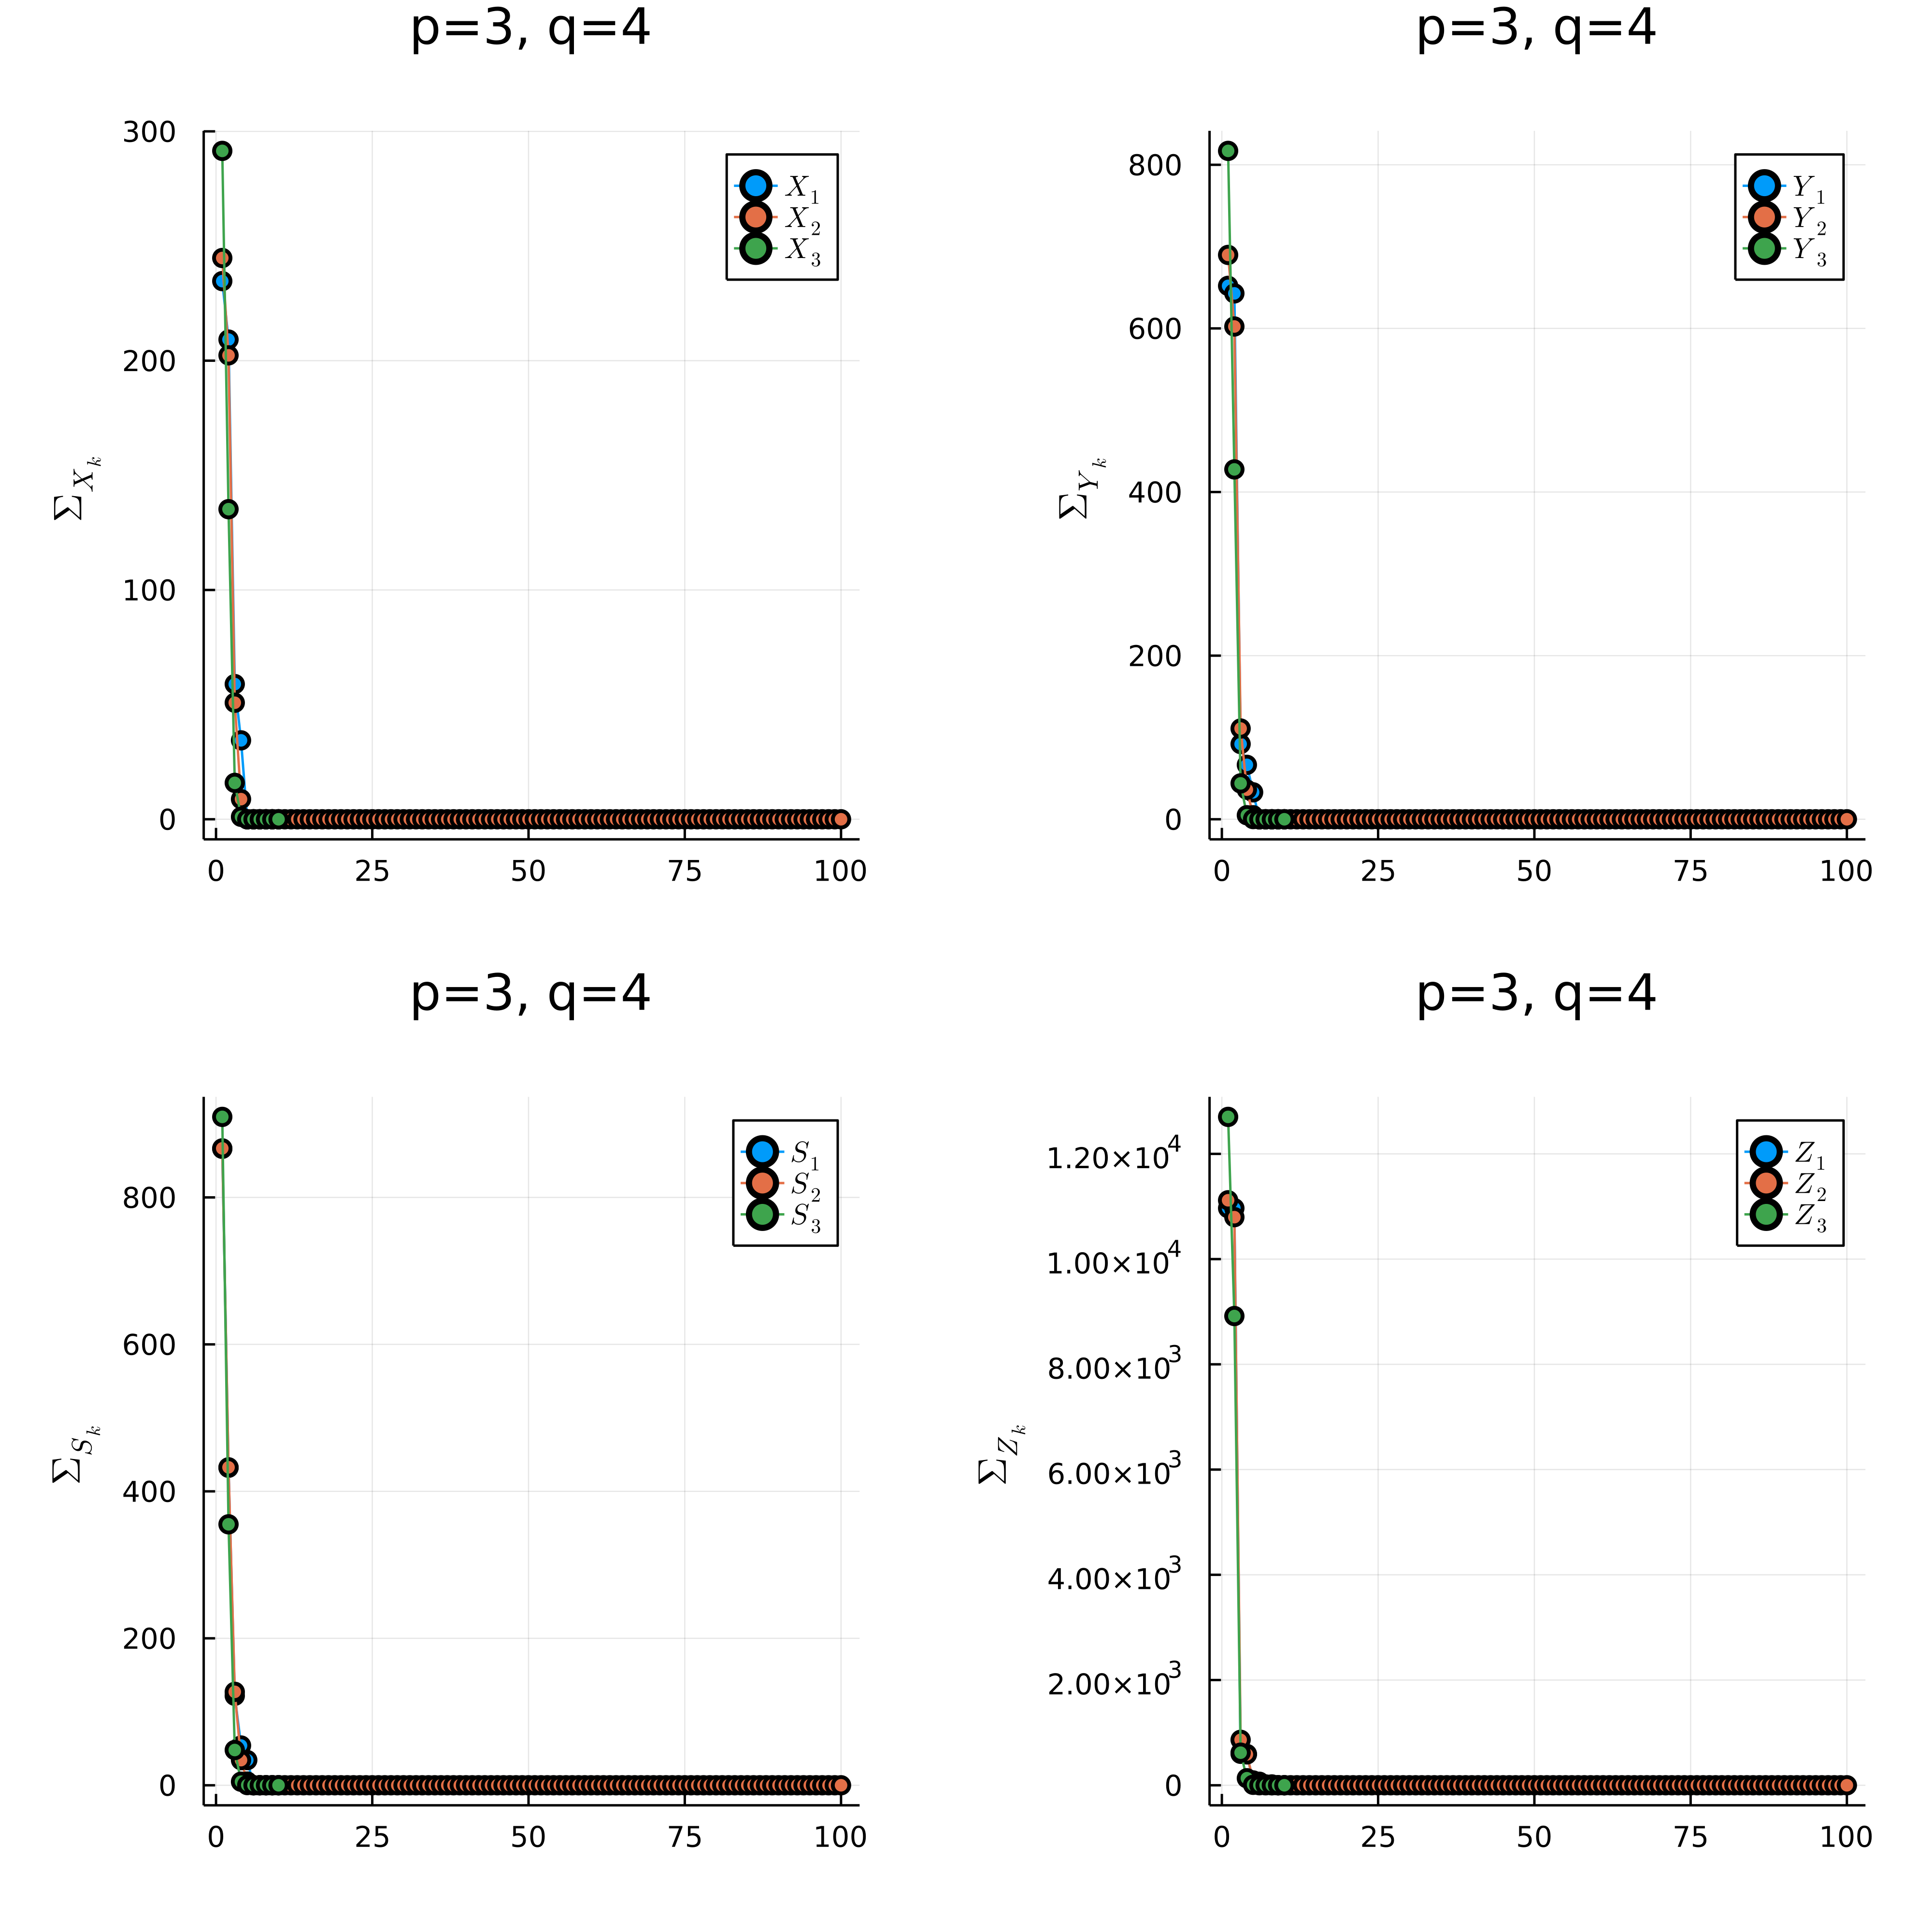
\includegraphics[width=\textwidth]{./plots/sigma_34.png}
    \caption{Some text}
\end{figure}

\begin{figure}[H]
    \centering
    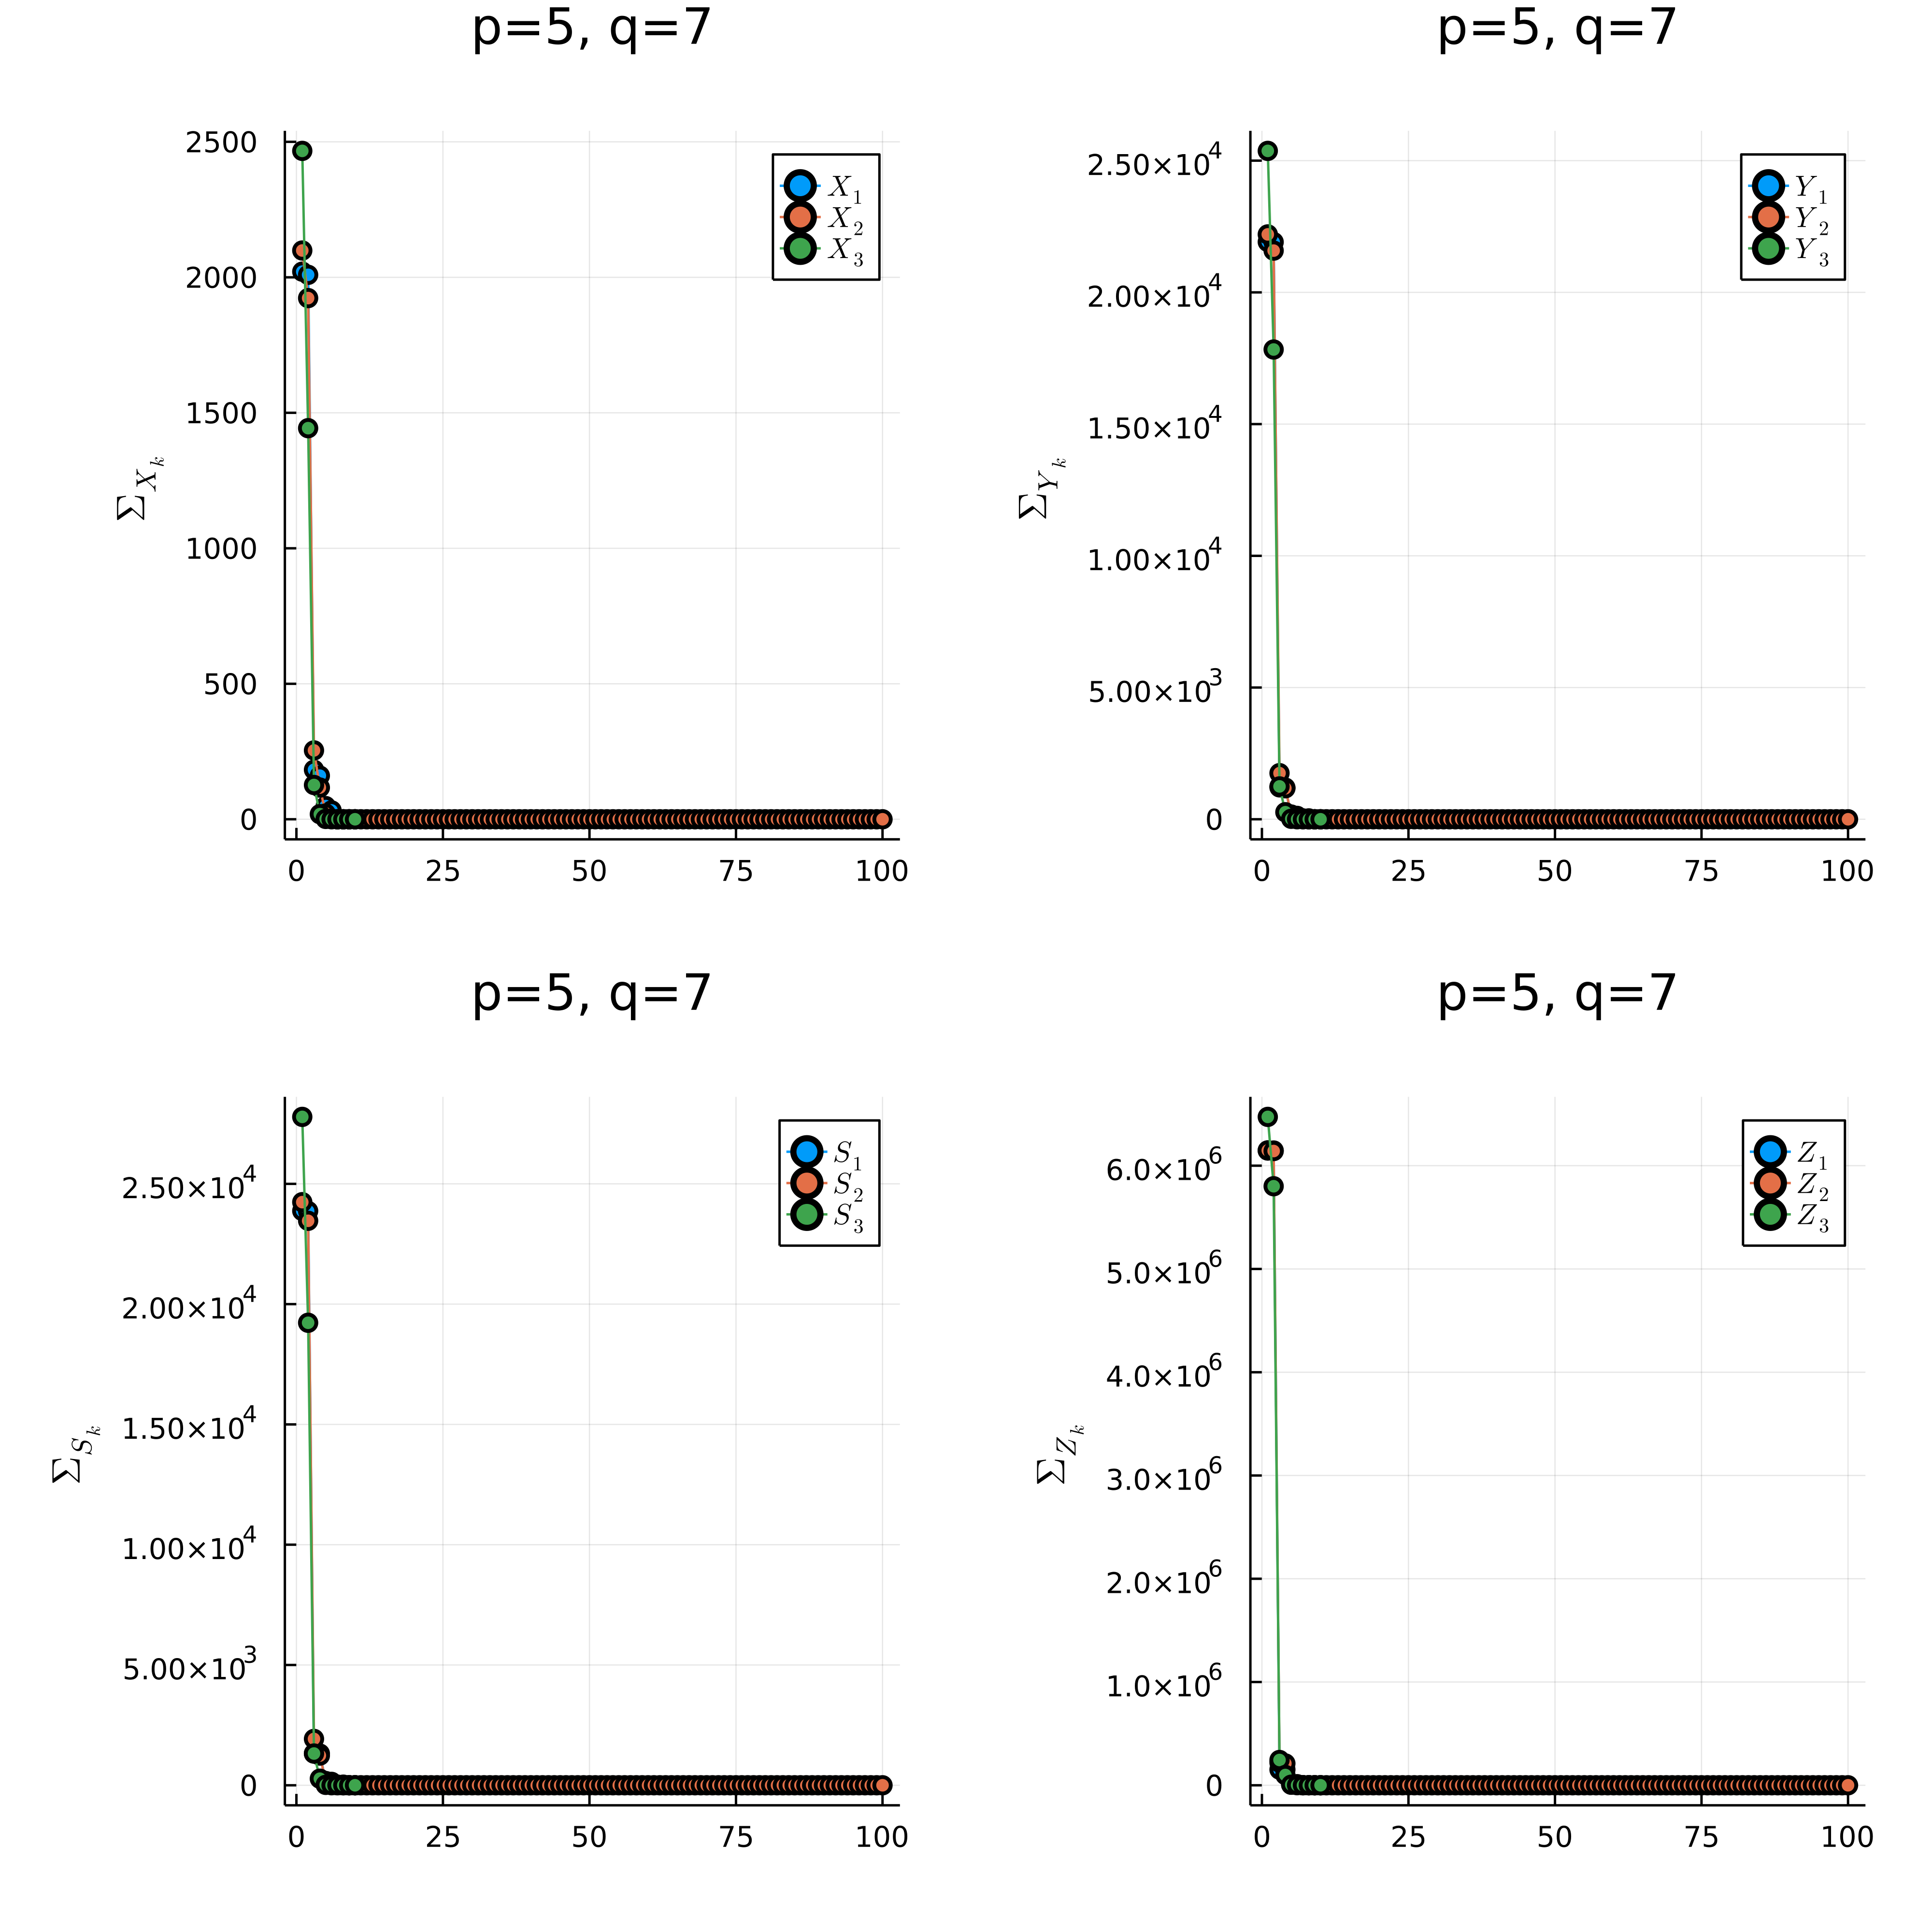
\includegraphics[width=\textwidth]{./plots/sigma_57.png}
    \caption{Some text}
\end{figure}

The following figures show the ranks MPS-TT unfolding matrices of $X, Y, S,
Z$ for $(p, q) = 3,4$ and $(p, q) = 5,7$ respectively

\begin{figure}[H]
    \centering
    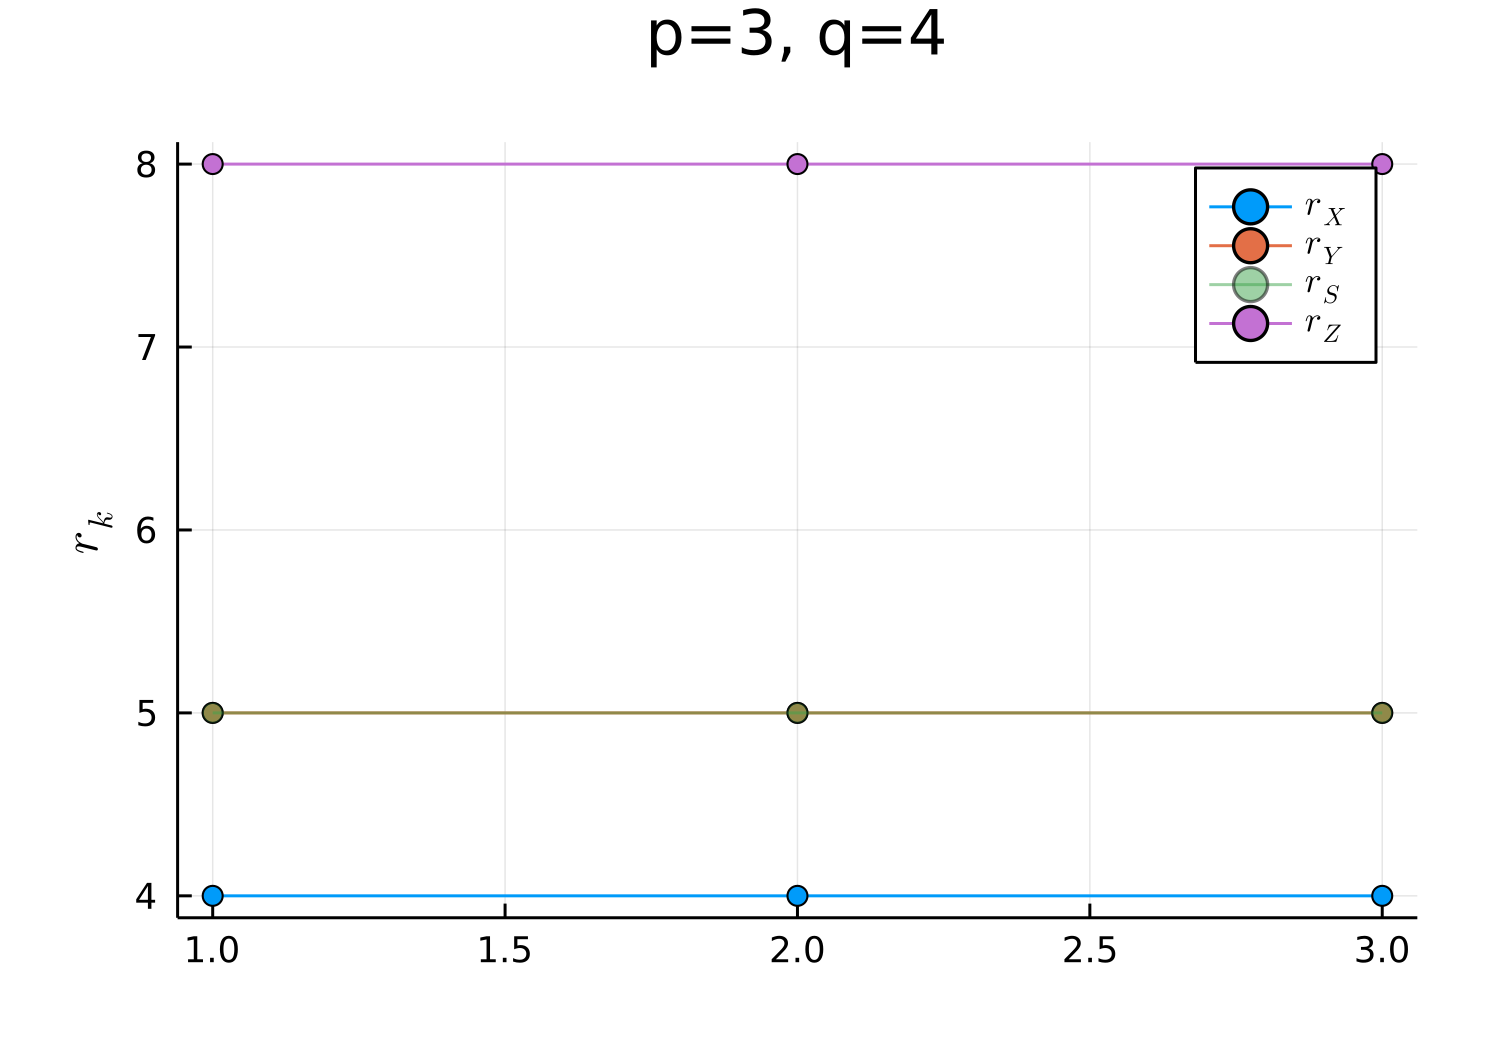
\includegraphics[width=0.48\textwidth]{./plots/rank_34.png}
    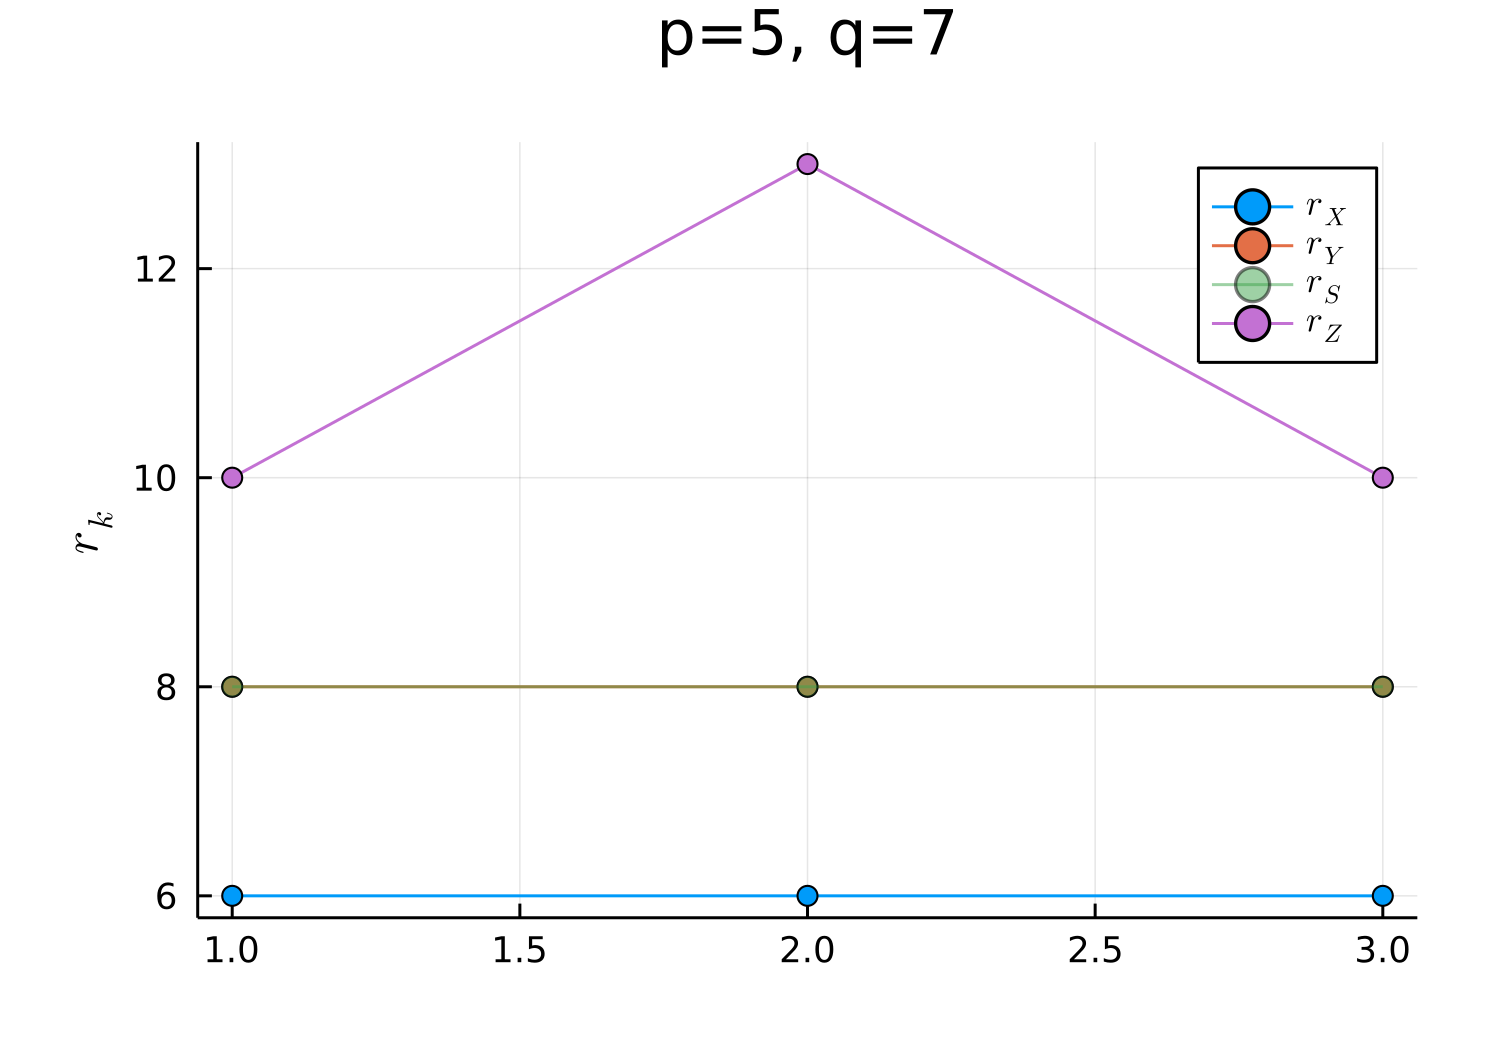
\includegraphics[width=0.48\textwidth]{./plots/rank_57.png}
    \caption{Some text}
\end{figure}
\nocite{code}
\printbibliography
\end{document}
